%-*- mode: LaTex; outline-regexp: "\\\\section\\|\\\\subsection";fill-column: 80; -*-
\documentclass[12pt]{article}
\usepackage[longnamesfirst]{natbib}
\usepackage[usenames]{color}
\usepackage{graphicx}  % Macintosh pdf files for figures
\usepackage{amssymb}   % Real number symbol {\Bbb R}
\usepackage{amsmath}
\usepackage{bbm}
\input{../../standard}

% --- margins
\usepackage{../sty/simplemargins}
\setleftmargin{1in}   % 1 inch is NSF legal minimum
\setrightmargin{1in}  % 1 inch is NSF legal minimum
\settopmargin{1in}    % 1 inch is NSF legal minimum
\setbottommargin{1in} % 1 inch is NSF legal minimum

% --- Paragraph split, indents
\setlength{\parskip}{0.00in}
\setlength{\parindent}{0in}

% --- Line spacing
\renewcommand{\baselinestretch}{1.5}

% --- page numbers
\pagestyle{empty}  % so no page numbers

% --- Hypthenation
\sloppy  % fewer hyphenated
\hyphenation{stan-dard}
\hyphenation{among}

% --- Customized commands, abbreviations
\newcommand{\TIT}{{\it  {\tiny Featurizing Text (DRAFT, \today)}}}
\newcommand{\prs}{\mbox{$\ol{\ol{R}}^2$}}

% --- Header
\pagestyle{myheadings}
\markright{\TIT}

% --- Title

\title{ Featurizing Text: Converting Text into Predictors for
            Regression Analysis }
\author{
        Dean P. Foster\footnote{Research supported by NSF grant 1106743} 
        \ \ Mark Liberman 
        \ \ Robert A. Stine\footnotemark[\value{footnote}]   \\
        Department of Statistics                             \\
        The Wharton School of the University of Pennsylvania \\
        Philadelphia, PA 19104-6340                          
}

\date{\today}

%%%%%%%%%%%%%%%%%%%%%%%%%%%%%%%%%%%%%%%

\begin{document}
\vspace{-0.5in}
\maketitle 
%------------------------------------------------------------------------
\vspace{-.5in}
\abstract{  

 Modern data streams routinely combine text with the familiar numerical data
 used in regression analysis.  For example, listings of real estate combine
 the price with a verbal description.  Some
 descriptions include numerical data, such as the number of rooms, but many others only verbally describe the property, often using an idiosyncratic vernacular. To exploit such data, we describe several
 techniques that that convert  text into numerical features suitable for
 regression analysis.  The proposed unsupervised techniques create features
 directly from text, requiring minimal user input. Because the constructions are unsupervised, the resulting features perform like typical regressors.  The techniques range from naive
 to subtle.  One can simply use raw counts of words, form principal components
 from these counts, or build regressors from counts of adjacent words.  Several examples illustrate the surprising success of
 these methods.  To partially explain this success, we take advantage of generating models developed for Bayesian analysis.  Because regressors derived from text are difficult to
 interpret, we also show how to develop interpretive hooks from incomplete quantitative features.

}

%------------------------------------------------------------------------
\vspace{0.15in}

\noindent
{\it Key Phrases:  latent semantic analysis, random projection, singular value decomposition, text mining, topic models} 

\clearpage

% ----------------------------------------------------------------------
\section{Introduction}
\label{sec:intro}
% ----------------------------------------------------------------------


\begin{description}



\item{Implications of Montanari}  Can you find little components?  

\item{Heuristic for ordered search} Since the higher indexed SVD components have little variation, Montanari's results suggest these may be below the noise floor.  That would explain, for example, why we don't see much signal from these in the sense that a full stepwise search focuses on those among the first 100. Though only heuristic (we have a richer environment), it does provide further motivation for the ordered search via AIC.  Also, what is $n$ for the modeling?  The number of tokens, or the number of documents.

\item{Parts of speech}  The plan is (a) find the nouns (b) remove the other words (c) redo the modeling.  Does the use of parts of speech help?

\item{Bigrams} Less useful here, though valuable in the identification of parts of speech as used in the prior step.  Bigrams (as in Dean's figure) identify syntactically similar words, which is a less useful context in our modeling as we demonstrate.  You can do more to build features that are predictive (earlier version of manuscript), but still don't match up to what we obtain from LSA.


\item{Relate to topic models} \\ 
 Simulation

\item{Variable selection}  \\
 AIC and connection to CV analysis.  Plot of reflections.

\item{Discussion}  \\
Lighthouse variables combine regular expression variables and linguistic variables. Other applications to wine.

\end{description}

 
 Software packages, such as (very elaborate, comprehensive) those in R
 \citep[tm][]{feinerer08} or Stanford NLP or openNLP.

 stopwords... ``and'', ``for'', ``in'', ``is'', ``it'', ``not'', ``the'', ``to'')
 
 \clearpage


 Modern data streams routinely combine text with numerical data.  For example,
 patient medical records combine lab measurements with physician comments.
  Analogously, online product ratings shown at Amazon blend explicit
 characteristics with verbal commentary.  How can one easily incorporate the
 information in such text into a model that predicts patient outcomes or product
 ratings?  Our objective here is to describe several particularly
 straightforward techniques for featurizing text, turning text into numerical
 variables suitable for regression modeling.
 
 
 As a specific example, we build a regression that predicts advertised prices
 of real estate properties from their listings.  Our data describe $n=$7,384
 property listings for Chicago, IL, extracted (with permission) from trulia.com
 on June 12, 2013.  At the time, trulia.com showed 30,322 listings for Chicago,
 but most were foreclosures that we excluded from our analysis.  The response in
 our models is the log of the listed price.  The distribution of the listed
 prices is right skewed, so we transformed the response to a log scale as shown
 in Figure \ref{fig:prices}.  The log transformation produces a roughly Gaussian
 distribution, with a hint of fat tails for produced by inexpensive properties
 with prices near \$25,000.  (This display uses the base 10 log of the prices
 for easy interpretation; subsequent models use natural logs.)
 
 
 \begin{figure}
 \caption{ \label{fig:prices} { \sl The distribution of prices for real estate
 in Chicago is highly skewed.  A log transformation produces data that are
 nearly normal.}  }
 \centerline{
 \vspace{0.1in}
 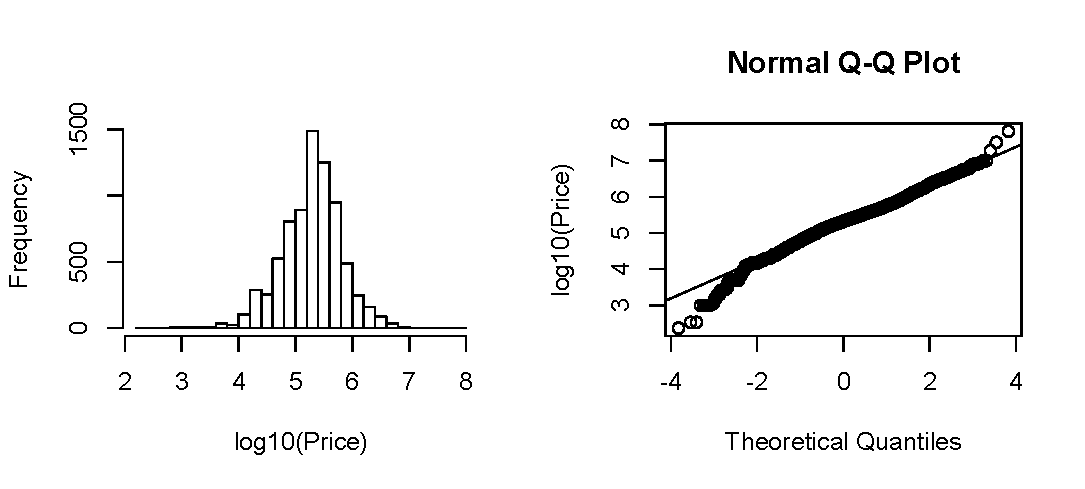
\includegraphics[width=5in]{figures/prices} }
 \vspace{0.2in}
 \end{figure}


 The listings that describe these properties are verbal, written in an
 idiosyncratic vernacular familiar only to those who are house hunting.  Some
 listings contain quantitative characteristics, but many do not.  The 
 following four listings are typical.  The initial value is the listed price.

 \begin{verbatim}
    $399000 Stunning skyline views like something from a postcard are yours
    with this large 2 bed, 2 bath loft in Dearborn Tower!  Detailed
    hrdwd floors throughout the unit compliment an open kitchen and
    spacious living-room and dining-room /w walk-in closet, steam
    shower and marble entry.  Parking available. 

    $13000 4 bedroom, 2 bath 2 story frame home. Property features a
    large kitchen, living-room and a full basement. This is a Fannie Mae
    Homepath property. 

    $65000 Great short sale opportunity...  Brick 2 flat with 3 bdrm
    each unit. 4 or more cars parking. Easy to show. 

    $29900 This 3 flat with all 3 bed units is truly a great
    investment!! This property also comes with a full attic that has
    the potential of a build-out-thats a possible 4 unit building in a 
    great area!!  Blocks from lake and transportation. Looking for a
    deal in todays market - here is the one!!! 
 \end{verbatim}

 \noindent
 Listings do not obey the grammatical rules of English.  Some authors write in
 sentences, others not, and a variety of abbreviations appear.  Punctuation
 varies from spartan to effusive (particularly exclamation marks), and the
 length of the listing runs from several words to a long paragraph.  The average
 listing has 73 words. The distribution of the lengths is right skewed; the
 shortest listing has 2 words whereas the longest has 568 words.  This variation
 in the lengths of the descriptions suggests that modeling the prices from this
 text requires some form of weighting: we simply do not know much about
 properties with short descriptions.

  
 A natural approach for a statistician confronted with such data is to construct
 intuitively appealing regressors from the listings.  For example, one might
 conjecture that an agent has a lot more to say about an expensive property than
 one in need of repair.  Hence, the length of a listing may be predictive of its
 price.  In a different vein, one can use regular expressions -- pattern
 matching -- to extract specific numerical data from the listings.  For example,
 the first listing indicates that this property has two bedrooms and two
 bathrooms.  A regular expression can be designed to extract numbers that
 precede the word ``bath'' from the listings.  Constructing such regular
 expressions, however, is a labor-intensive process that must be done on a
 case-by-case basis.  The patterns become complex because they must allow common
 abbreviations, such as ``bth'', ``bath'' and ``bthrm'' in order to match counts
 of the number of bathrooms.  Complexity aside, the greater problem with
 explicit pattern matching is that most listings omit these characteristics.
  The only numerical data common to every listing is the response, the
 advertised price.  For these listings, our regular expressions found that 6\%
 of the listings indicate the number of square feet, 26\% indicate the number of
 bathrooms, and 42\% give the number of bedrooms.  More complex regular
 expressions would likely find more matches, but the gains are likely to be few.
  As illustrated next, one faces a Type I/Type II trade-off.  Simple regular
 expressions miss some matches, but more aggressive expressions match
 inadvertently.


 The four scatterplots in Figure \ref{fig:parsed} summarize the marginal
 association between the log of prices and these constructed predictors,
 including the number of words in descriptions.  For listings with no match, we
 filled the missing values with the averages of the observed cases.  These
 appear as columns of gray points located at the mean of each variable on the
 $x$ axes in Figure \ref{fig:parsed}.  The correlations between these variables
 and the log of the prices vary from moderate to nearly zero.  The length of the
 listing has the largest correlation with log prices ($r=0.40$). The frame that
 shows this association includes the fit of a fifth-order polynomial that
 recovers the evident nonlinearity of this association.  The nonlinearity is
 highly significant, but increases the amount of explained variation from 0.16
 to only 0.20.  The improvement in fit is slight because most of the data lie
 within the linear range of the fit.  Missing data has a large impact on the
 correlations with the other extracted features shown in Figure
 \ref{fig:parsed}.  The correlations for complete cases are 0.42 for the number
 of bathrooms, 0.26 for the log of the number of square feet, and 0.09 for the
 number of bedrooms.  If missing data are included, the correlations become much
 smaller (the second correlation shown in each frame).  These plots also show
 several anomalies.  For example, the scatterplot of the log price on log length
 shows a cluster of 25 listings, all with exactly 265 words (log 265=5.6).
  These are not errors: All of these different properties were listed with a
 common format by a government agency.  The scatterplot of the log of prices on
 the log of the square footage also shows a clear outlier; this outlier is a
 consequence of aggressive matching in a regular expression.  A typo in a
 description (``has 1sfam'') led our regular expressions to find a property with
 1 square foot.

 \begin{figure}
  \caption{ \label{fig:parsed} { \sl Extracted characteristics have moderate to
 slight positive association with the log of the prices. } Gray points in the
 figures identify cases that omit the explanatory variable; the first shown
 correlation in each frame uses only the observed data; the following smaller 
 value includes mean-filled listings. }
 
\centerline{
 \vspace{0.1in}
 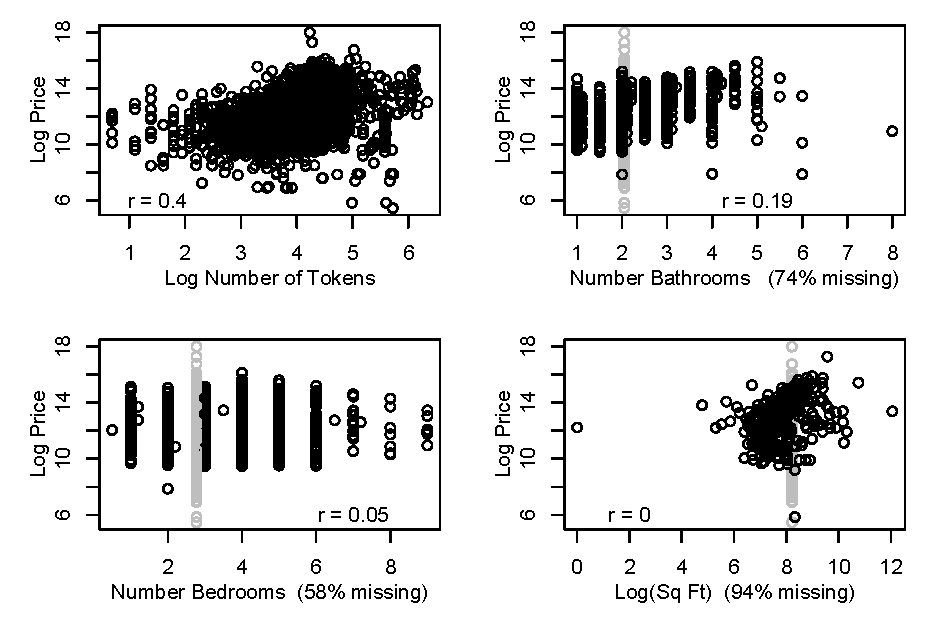
\includegraphics[width=5in]{figures/parsed} }
 \vspace{0.2in}
 \end{figure}


 Table \ref{tab:parsed} summarizes the fit of a regression of the log of price
 on predictors built from the four extracted features. The model includes a
 fifth-degree polynomial in the log of the length of the description and missing
 data indicators.  These indicators are coded as 1 when the associated regular
 expression found a match and are coded as 0 otherwise.  Aside from the
 components of the polynomial, the features are not highly collinear, and the
 multiple regression echoes the marginal associations observed in Figure
 \ref{fig:parsed}.  Features related to the lengths of listings explain the most
 variation, followed by the number of bathrooms.  Unlike the marginal
 associations, the log of the number of square feet and its missing indicator
 are highly significant.  The missing indicators for bedrooms and bathrooms are
 not.  The model explains about one-fifth of the variation in prices;  
 if adjusted for prediction, the predictive R-squared \citep{fosterstine14b} is
 \begin{equation}
   \prs = 1 - \frac{\mbox{RSS}/(n-2p)}{\mbox{TSS}/(n-1)} = 0.231.
 \end{equation}
 \prs adjusts for the effects of estimation when predicting out-of-sample.

 
 \begin{table}[ht]
\caption{ \label{tab:parsed} {\sl OLS multiple regression of log prices on the
 parsed explanatory variables and  indicators of observed values.}}
\centering
\begin{tabular}{lrrrr}
  \hline
    Feature       & Estimate & Std. Error & t value & Pr($>$$|$t$|$) \\ 
  \hline
  Intercept       & 7.9985 & 0.4749 & 16.84 & 0.0000 \\ 
  log Tokens      & 39.0183 & 1.0945 & 35.65 & 0.0000 \\ 
  $(\mbox{log Tokens})^2$   & 1.0086 & 1.0642 & 0.95 & 0.3433 \\ 
  $(\mbox{log Tokens})^3$ & -18.2556 & 1.0612 & -17.20 & 0.0000 \\ 
  $(\mbox{log Tokens})^4$ & -4.8956 & 1.0594 & -4.62 & 0.0000 \\ 
  $(\mbox{log Tokens})^5$ & 7.9094 & 1.0584 & 7.47 & 0.0000 \\ 
  log Sq Feet     & 0.4039 & 0.0579 & 6.98 & 0.0000 \\ 
  Sq Feet obs     & 0.6254 & 0.0594 & 10.53 & 0.0000 \\ 
  Bedrooms        & 0.0080 & 0.0165 & 0.48 & 0.6299 \\ 
  Bedrooms obs    & -0.0084 & 0.0299 & -0.28 & 0.7783 \\ 
  Bathrooms       & 0.4015 & 0.0300 & 13.37 & 0.0000 \\ 
  Bathrooms obs   & -0.0199 & 0.0336 & -0.59 & 0.5537 \\ 
   \hline
   \multicolumn{5}{c}{\prs = 0.231, \; $s_e = 1.06$}\\
   \hline
\end{tabular}
\end{table}

 
 
 Had listings been composed in a consistent manner with a standardized set of
 characteristics, such constructive modeling would surely be more successful.
  Our goal here takes us in a different direction that, in contrast to this
 constructive approach, explores automatic methods that thrive in this
 unformatted, irregular context.  These methods are collectively known as {\em
 vector space models} in computational linguistics \citep[e.g.][]{turney10}.  A
 vector space model (VSM) characterizes each document as a point in some
 $p$-dimensional vector space, typically \Rp.  VSMs originated in artificial
 intelligence and were adopted for text applications to construct a system for
 document retrieval known as latent semantic indexing \citep{deerwester88}.
  Latent semantic indexing generates clusters of documents to enable a query to locate
 related items.  VSMs are closely related to techniques that statisticians will
 find familiar: principal components analysis (PCA) and canonical correlation
 analysis (CCA).  The underlying computational engine is a singular value
 decomposition (SVD), aided by random projections.  (The use of the SVD
 occasionally leads to VSMs being described as ``spectral algorithms'' which
 should not be confused with frequency domain methods for time series.)  There
 has been considerable debate as to how VSMs represent language; we leave to
 linguistics the task of explaining why such simple representations of text
 might capture deeper meaning \citep{deerwester90, landauer97, bullinaria07,
 turney10}.


 VSMs are commonly found in unsupervised applications such as clustering, but
 our application here finds that they are equally effective in supervised
 models.  In essence, each document is represented as a point in \Rp, and these
 coordinates become regressors.  These regressors can be used alone or in
 combination with traditional variables, such as those obtained from a lexicon,
 regular expression, or semantic model.  The example of real estate listings
 illustrates the impact of various choices on the predictive accuracy.  For
 example, a regression using the automated features produced by a simple VSM
 explains over two-thirds of the variation in listed prices for real estate in
 Chicago.  The addition of several substantively derived variables adds little.
  Though we do not emphasize its use here, variable selection can be employed to
 reduce the ensemble of regressors without sacrificing predictive accuracy.  An
 application that models personality traits derived from Facebook messages
 appears in \citet{ungar13}.


 The remainder of this paper develops as follows.  The next section reviews
 latent semantic analysis (LSA) and uses this method from
 computational linguistics to featurize text.  LSA corresponds to
 principal components regression.  Section \ref{sec:tokenspace} presents vector
 space models such as LSA from from the novel perspective that we call ``token
 space.'' Token space characterizes text as points in a very high dimensional
 space that restores the statistical sense of ``observations,'' samples drawn
 from a population.  In token space, LSA is seen to correspond to a CCA between
 words and the context of those words.  Various definitions of the context of a
 word allow one to construct many types of features.  Though 
 simple to describe, it is more subtle to appreciate why a VSM works in
 regression.  Section \ref{sec:topic} offers one explanation by relating VSMs to
 a topic model that reproduces many aspects of the real estate listings.
  Section \ref{sec:cv} returns to regression models for real estate with a
 discussion of the use of variable selection and uses cross-validation to
 measure the success of methods and to compare several models.  Variable
 selection is particularly relevant if one chooses to search for nonlinear
 behavior.  We close in Section \ref{sec:disc} with a discussion and collection
 of future projects.



%--------------------------------------------------------------------------
\section{Featurizing with Latent Semantic Analysis}
\label{sec:lsa}
%--------------------------------------------------------------------------

 LSA is essentially principle components analysis
 of a matrix whose elements count how often each word appears in a document (in our
 case, the frequency of words in a property listing).  Using these components as
 features in regression then amounts to a principle components regression.
  Quite a few details, however, need to be resolved in any application. For
 example, what is a word?  How should the data be scaled? 
 This section describes the relevant choices within
 the context of building a regression model for real estate prices.
 
 \subsection{ Tokenization }  % ------------------

 LSA begins by converting the source text into {\em word tokens}.  A word token
 is a sequence of one or more characters that represents an instance of a unique
 {\em word type}.  This conversion of text into tokens is known as tokenization.
  Tokenization requires making numerous, often subtle, choices.  For example, is
 the number ``735'' a word token?  Do the tokens ``state'' and ``State''
 represent the same word type?  Are ``room'' and ``rooms'' instances of the same word
 type?  To answer these questions, we adopt a standard, simple approach: we
 convert all text to lower case, distinguish punctuation characters as separate
 types, and replace instances of rare word types by a common token.  To
 illustrate some of the issues, consider the following listing:
 \begin{verbatim}
   Brick flat, 2 bdrm.  With two-car garage. \end{verbatim} 
 \noindent
 Separated into tokens, this text becomes a list of 10 tokens representing 9
 word types (angle brackets surround punctuation tokens)
 \begin{verbatim}
   {brick, flat, <,>, 2, bdrm, <.>, with, two-car, garage,<.> } \end{verbatim} 
 \noindent
 We leave embedded hyphens in place and do not correct spelling errors and
 typos.  Abbreviations remain as given.  References such as the texts by
 \citet{manning99} and \citet{jurafsky09} describe more elaborate choices, such
 as stemming and annotation, that can be incorporated into
 tokenization. \citet{turney10} give a concise overview.  Notice that
 tokenization only distinguishes word types, not  meaning or use
 (does not distinguish homographs). A variety of open source platforms are
 available for processing natural language, such as the freely-available NLTK 
 package \citep[][ and on-line at http://www.nltk.org]{nltk09}.

  
 When applied to our data from Chicago, the 7,384 property listings contain
 536,485 word tokens representing 15,227 unique word types.  As usual in text,
 the most common word types occur frequently whereas most words appear
 infrequently.  More than half of these tokens appear only once or twice,
 providing little exposure to how the word is used.  We clustered these rare
 types into one category ($<$OOV$>$, for ``out of vocabulary''), resulting in a
 reduced vocabulary of $m = 5,707$ word types.  The most common word types are
 punctuation: `.'  occurs 40,227 times and `,' occurs 33,746 times.  Following
 these come the collection of seldom seen word types (OOV, 11,478), `and'
 (frequency 11,032), `!' (7,894) and `in' (7,418).  Figure \ref{fig:zipf} graphs
 the log of the frequency of these word types versus the log of their ranks.  It
 is common in text to find a linear trend with slope near 1 in this graph, the
 signature of a Zipf distribution \citep{zipf35, baayen02}.  In that case, the
 rank of a word type times its frequency would be constant.  Even though the
 text of real estate listings is not standard English, one expects to find
 counts resembling those produced by a power law \citep{clauset09}.  The shown
 line (with log-log slope -0.927) holds only for more common word types.  For
 less common words (here, outside the most common 500 words), the frequencies
 drop off more rapidly.  (This change in slope is also seen for words in
 Wikipedia.)


 \begin{figure}
 \caption{ \label{fig:zipf} { \sl The log of the frequency of word types in the
 listings for properties in Chicago is roughly linear in the log of the rank of
 the words.}  The shown line $\log \mbox{freq} = 10.9 - 0.93 \log \mbox{rank}$ 
 was fit to the most common words with ranks 1 through 500.  }

 \centerline{
 \vspace{0.1in}
 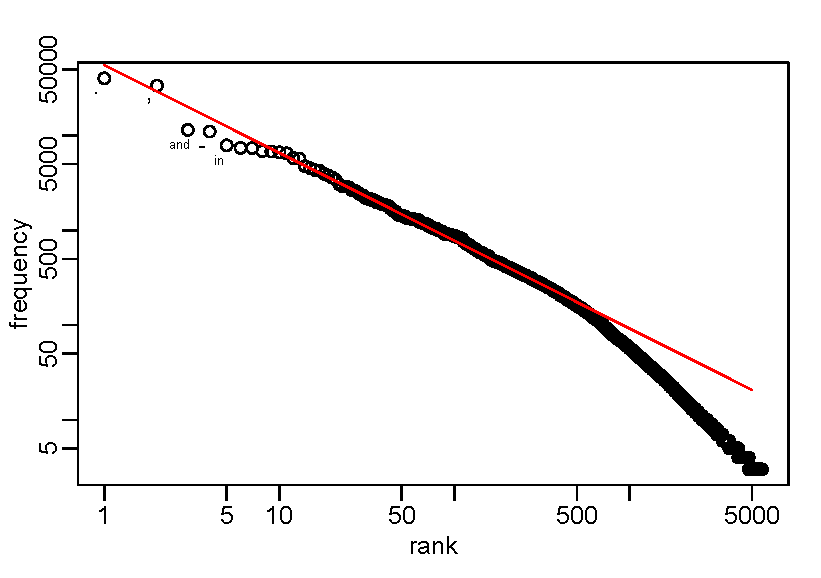
\includegraphics[width=3.5in]{figures/zipf} }
 \vspace{0.2in}
 \end{figure}


 Once the source text has been tokenized, we collect counts of how often each
 type appears within a listing.  These counts treat each listing as a ``bag of
 words,'' a multiset that does not distinguish the placement of words within a
 listing.  Permuting the words within a listing produces the same counts.  Let
 $n$ denote the number of listings; we treat each listing as an observation in
 the usual sense.  Let $V$ denote the vocabulary, the set of $m$ distinct word
 types.  The $n \times m$ context-word matrix $W$ holds the counts of these word
 types across the listings; $W_{ij}$ is the number of times word type $j$
 appears in the \ith document.  (All vectors in our notation are column
 vectors.)  (The transpose of $W$, often called the term-document matrix, is
 common within computational linguistics. We follow the convention within
 statistics and arrange observations -- the listings -- as rows. In our context
 a listing is a document.)  The matrix $W$ is sparse: a small portion of the
 vocabulary appears in most listings. We assume that the columns of $W$ are
 sorted so that the first column $W_1$ holds the most frequent word type, the
 second column $W_2$, holds the second most frequent, and so forth.


\subsection{ Regressing on Word Types }  % ----------------------

 Before turning to LSA, we fit models directly on the frequencies in $W$.
  Because LSA constructs features that are linear combinations of the columns of
 $W$, all of the signal captured by LSA lies within $W$.  By regressing log
 prices directly on $W$, we can bound how much variation LSA can explain.  Our
 fits of log price on $W$ adjust for the lengths of the listings.  As shown in
 Figure \ref{fig:parsed}, the length of a listing is correlated with its price.
  Keeping this polynomial in length in the regression implies that, for a word
 to be a significant predictor, its association with price must run deeper than
 its incremental contribution to the length.  Starting from this initial
 polynomial, we accumulated the $R^2$ statistic as first 3,000 columns of $W$
 join the model.  The solid curves in Figure \ref{fig:cumr2} track $R^2$ as
 these frequencies are added in either decreasing order (upper curve, for adding
 $W_1,W_2,\ldots,W_{3000}$) or increasing (lower curve, for $W_{3000},
 W_{2999},\ldots, W_1$) frequency.  The gap between these curves and concave
 shape of the upper curve show that adding more frequent words first achieves a
 better fit with fewer variables. This figure also shows the degree of
 collinearity within $W$.  PCA is useless if applied to orthogonal
 variables. The sparsity of $W$ produces small correlations between pairs of columns
 of $W$, but collinearity emerges over larger collections.  For example, when
 adding features in order of decreasing frequency, 219 of these counts of 3,000 word types
 were redundant (representable as linear combinations of others).  To illustrate
 the effects of this collinearity in regression, the dashed curve in Figure
 \ref{fig:cumr2} shows the contribution to $R^2$ of words in order of decreasing
 frequency, but with the magnitude of the change in $R^2$ as if added in the
 other order.  For example, when added after
 $W_1, \, W_2,$ and $W_3$, adding the count of OOV tokens ($W_4$) boosts $R^2$ by about 0.02.  If added after $W_{3000},\,W_{2999}, \ldots, W_5$, the frequency of OOV
 tokens adds much less to the fit, contributing only 0.0003 to $R^2$.  Were there 
 no collinearity, the improvements to $R^2$ would match, and the dashed curve in Figure \ref{fig:cumr2} would lie on top of the upper solid curve. 

\begin{figure}
\caption{ \label{fig:cumr2} 
{\sl Accumulated $R^2$ statistics of regression models with word frequencies
 added in order of decreasing (top solid black) or increasing (lower solid
 black) frequency.} The dashed curve shows the contributions having adjusted for
 subsequent words and illustrates the effects of collinearity among the word
 counts.}  
 \centerline{ 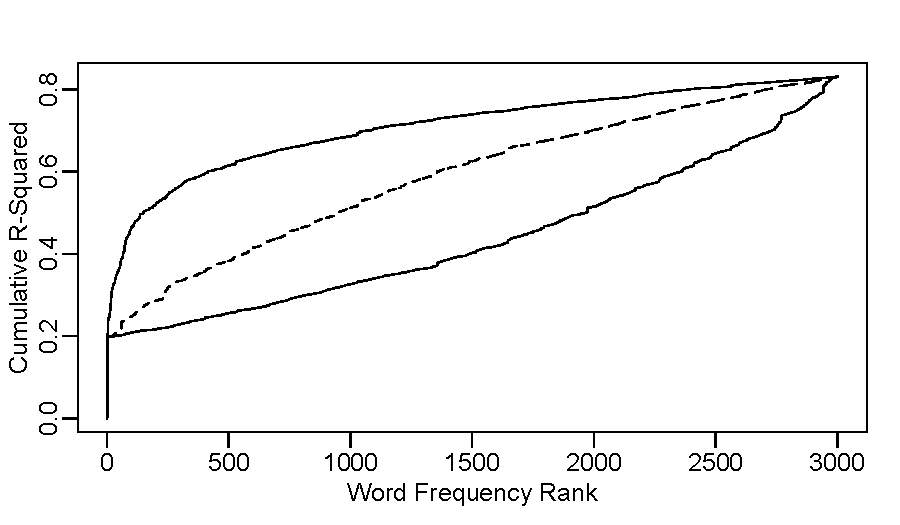
\includegraphics[width=4in]{figures/cumr2.pdf} }
\end{figure}


 The slow growth of $R^2$ after the first hundred or so frequencies suggests
 that later features add too much noise to the fit and degrade predictions.  
 Even so, a model that simply adds the 3,000 most frequent words to
 the baseline polynomial in document length provides a statistically significant 
 improvement. Adding
 $W_1,\ldots,W_{3000}$ improves $R^2$ from 0.194 to 0.832, a highly significant
 increase.  Nonetheless, the resulting model is huge relative to the number of
 observations and has many insignificant estimates.  One has numerous approaches
 to trimming its size, such as shrinkage or subset selection.  Because the word
 frequencies are correlated but easily ordered (by frequency), we use the
 corrected AIC statistic \citep{hurvich89}
 \begin{equation}
    AIC_{c}(k) = n \log \frac{RSS(k)}{n} + \frac{n+k}{1-(k+2)/n} \;,
 \end{equation}
 where $k$ is the number of estimated parameters in the regression.  Rather than
 try to pick the best subset -- which would require a strong penalty against
 over-fitting -- we use $AIC_c$ to pick the best stopping point in the 
 sequence of models determined by word frequency, much as one might pick the
 order of an autoregression.  Figure \ref{fig:aic} graphs $AIC_c$ for the
 sequence of models obtained by adding words in order of decreasing frequency
 when added to the initial polynomial in the log of the length of the listings.
  The minimum of $AIC_c$ occurs with $k=1,089$ words, giving \prs = 0.580.
  Residual plots show fat tails (consistent with the distribution of log prices
 in Figure \ref{fig:prices}), but no evidence of heteroscedasticity that might
 be anticipated due to the differences among the lengths of the listings.

\remark{ The comparison of these models explains our preference for reporting
 \prs in the context of large regressions.  We want a model that predicts the
 price of a listing from its text.  For the regression chosen by $AIC_c$ with 1,089 words, 
  $R^2 = 0.705$ and $\ol{R}^2=0.654$.  The larger model 
 with 3,000 words reaches $R^2 = 0.832$, with $\ol{R}^2 = 0.719$.  Superficially,
 the more familiar $R^2$ and $\ol{R}^2$ both convey the impression that the larger
 regression is more predictive than the model chosen by $AIC_c$.  Predictive
 R-squared provides a more realistic evaluation of the ability of the large
 model to predict, namely its \prs = 0.15.}


\begin{figure}
\caption{  \label{fig:aic}  
  {\sl Corrected AIC for three regression models: regressors in one are words in order of
 decreasing frequency (dots), and those in the two others are computed from either
 LSA (solid) or bigrams (dashed).}  Small circles mark the positions of the
 minimum $AIC_c$ statistic for each sequence.}  
 \centerline{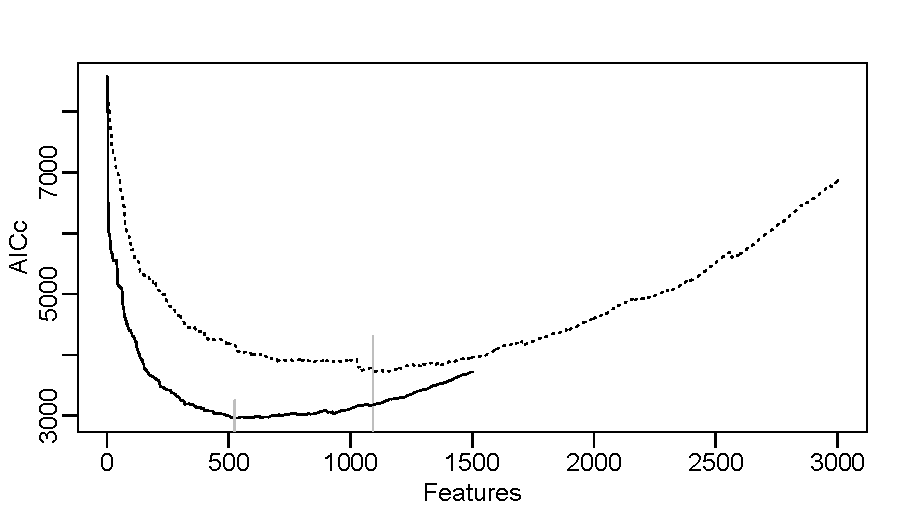
\includegraphics[width=4in]{figures/aic.pdf} }
\end{figure}


\begin{figure}
\caption{  \label{fig:wordtstats}  
  {\sl Absolute $t$-statistics from the regression of log prices on word
 frequencies for the model selected by $AIC_c$.}  In the left panel, the
 horizontal black line locates $\ev |Z|$ for $Z \sim N(0,1)$, the higher dashed
 line is the Bonferroni threshold, and the red curve is a loess smooth of $|t|$.
  In the right panel, the red line is fit to the smallest 20\% of the
 $|t|$-statistics, producing the shown slope.}  \centerline{
 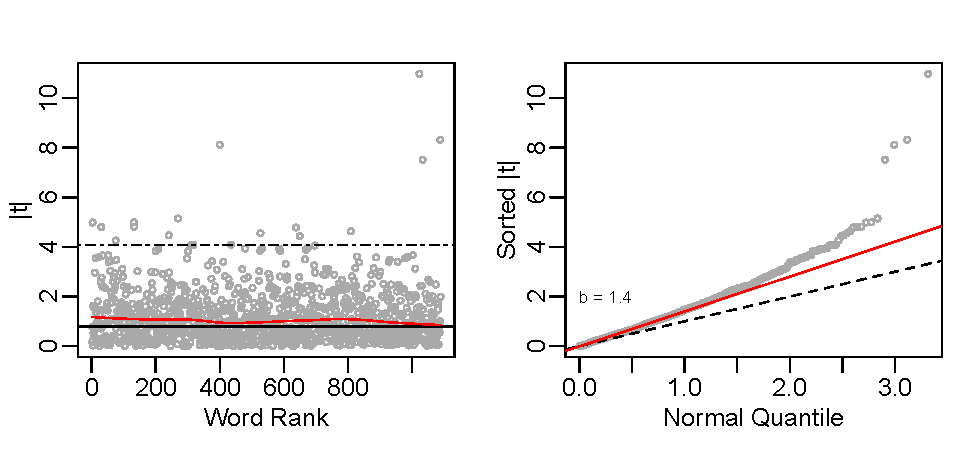
\includegraphics[width=5in]{figures/word_tstats.pdf} }
\end{figure}

 
 Although the model selected by $AIC_c$ explains a great deal of variation in
 prices, the signal remains diffusely spread over the words.  Few estimates
 stand out, leaving substantial signal embedded in the background.  Figure
 \ref{fig:wordtstats} summarizes the t-statistics in this fit. The left panel of
 the figure graphs $|t|$ for the words in order of decreasing frequency.  The
 solid horizontal black line is the expected value of the absolute value of a
 standard normal, $\sqrt{2/\pi}$. The dashed horizontal line is the Bonferroni
 threshold $\Phi^{-1}(1-0.025/1089) \approx 4.08$.  Between these, the almost
 flat, red curve is the loess smooth of $|t|$; the average $|t|$ is only slightly
 larger than one expects for a model with no signal.  Scattered coefficients of
 only 16 words exceed the Bonferroni threshold.  For example, the coefficient
 for the word ``vacant'' has $t=-8.1$; not surprisingly, the addition of this
 word to a listing lowers the expected price.  In contrast, the presence of
 additional out-of-vocabulary words predict higher than average prices
 ($t=5.0$).  Though these predictors stand out, a model limited to these clearly
 significant words has $R^2 = 0.236$, leaving much variation unexplained.  The
 half-normal plot in the right panel of Figure \ref{fig:wordtstats} confirms the
 diffuse signal: the fitted $t$-statistics are inconsistent with noise, but not
 by much.  The dashed line in the half-normal plot is the diagonal; the solid line
 is a regression fit to the smallest 20\% of the $|t|$-statistics.  For a sample
 from a standard normal distribution, the slope should be 1.  The slope of these
 estimates is significantly larger, but clearly the signal is widely spread over
 many words rather than concentrated in a few.
   

 \subsection{ Regressions using LSA }  % ------------------
 \label{sec:regrUsingLSA}
 
 The use of LSA to create features for regression models essentially reproduces
 principal components regression.  Rather than regress prices on column of $W$,
 regress prices on principal components of $W$.  The only differences from the 
 usual principal components regression are the absence of centering and the 
 variety of choices for weighting the frequency counts in $W$ prior
 to constructing the principal components.
 

 Three of the common choices for weights can be motivated as variance stabilization. 
 For example, one might choose to stabilize the differing variances produced by 
 unequal document lengths.  Define
 ${W}^{*}$ to be the $n \times m$ matrix with elements ${W}^{*}_{ij} =
 W_{ij}/\sqrt{n_i}$ with $n_i = \sum_j W_{ij}$ counting the number of word
 tokens in the \ith listing.  Were tokens within listings random samples from a
 multinomial distribution with probabilities $p_{1}, \ldots, p_{m}$ across the word types,
 then $\Var({W}^{*}_{ij}) = p_j(1-\sum_{k\ne j} p_k)$, regardless of the
 number of words in the listing.  Similarly, we can define $W^{**}$ with elements
 $W^{**}_{ij} = W_{ij}/\sqrt{m_j}$, where $m_j = \sum_i W_{ij}$ counts the
 number of tokens of word type $j$ across all listings. This standardization
 down-weights the most common word types.  Our choice for weights combines these and uses
  \begin{equation}
   \widetilde{W}_{ij} = W_{ij}/\sqrt{n_i\,m_j} \;.
  \label{eq:Wtij}
  \end{equation}
  This combination produces a novel approximation to a canonical correlation analysis developed in Section \ref{sec:cca} below. \citet{turney10} describes these and other weightings, such as the popular term frequency-inverse document
 frequency (TF-IDF),  used in LSA. 
  
  
 % The popular method known as  replaces the frequencies emphasizes less common 
 % word types and counts the number of
 % documents in which a word appears rather than its overall frequency.  For the
 % simplest version of TF-IDF, let $d_j = \sum _i\one{W_{ij} > 0}$ count the
 % number of listings in which word type $j$ appears and replace $W_{ij}$ by
 % $W_{ij} \log(n/d_j)$.  For instance, if the word type ``.'' appears in every
 % listing, then $d_j = n$ and $\log n/d_j = 0$, removing this ubiquitous type from the
 % construction of principal components. 
 
 
 Whichever weighting is selected, we compute the leading principal components of $W$ 
  by using random projections.
  Random projections produce accurate approximations to the truncated SVD of
 $W$ much more quickly than standard algorithms.  Though not absolutely necessary in this application -- one can compute
 the usual SVD of $W$ exactly -- random projections become necessary as
 the number of documents and size of the vocabulary grow.  Denote the SVD of the
 document-word matrix $W$ by
 \begin{equation}
       W = U D V' = \sum _{i=1}^{\min(m,n)} \la_i U_i V_i' \;,
 \label{eq:W}
 \end{equation}
 where $U = [U_1,\ldots,U_n]$ and $V=[V_1,\ldots,V_m]$ are orthonormal, and $D =
 \mbox{diag}(\la_i)$ is a $n \times m$ diagonal matrix, with the singular values
 $\la_1 \ge \la_2 \ge \cdots \ge \la_{\min(m,n)}$ along the diagonal.  The
 columns of $U$ are the eigenvectors of $XX'$ (the sought principal components,
 or left singular vectors), and the columns of $V$ are the eigenvectors of
 $X'X$.  The truncated, or thin, SVD zeros all but the largest, say, $k$
 singular values and produces an approximate factorization of $W$ that we denote
 \begin{equation}
       W_{1:k} \approx U_{1:k} D_k V_{1:k}' = \sum _{i=1}^k \la_i U_i V_i' \;,
 \label{eq:Wk}
 \end{equation}
 $U_{1:k}$ and $V_{1:k}$ hold the first $k$ columns of $U$ and $V$,
 respectively, and $D_k$ is the corresponding leading portion of $D$. We use the
 colon in a subscript to distinguish the matrix holding several columns from the
 columns themselves.  The computation of $U_{1:k}$ by direct means is relatively
 slow (a few hours of a current desktop computer), even for this problem with
 about 7,384 rows and 5,707 columns.  To speed this calculation, we exploit
 random projection algorithms defined and analyzed in \citet{tropp10}.  Random
 projections produce $U_{1:k}$ in less than a minute in our application and are
 essential in larger problems.

 
 Suppose in the ideal case that $W$ essentially has rank $k$ in the sense that
 $\la_k \gg 0$ and $\la_{k+1} \approx 0$.  Let $\ell$ denote an integer slightly
 larger than $k$ \citep[see][for the details]{tropp10}.  Form an $m \times \ell$
 matrix $\Omega_{\ell}$ with random elements $\Omega_{ij} \sim N(0,1)$,
 independently, and compute the product $A_{\ell} = (W W')^q W \Omega_{\ell}$
 for small $q$.  (We set $q = 4$.)  The initial multiplication of $W$ by
 $\Omega_\ell$ reduces the number of columns from $m$ to $\ell$; subsequent
 multiplication by $W W'$ improves the approximation, resembling the power
 method for finding eigenvalues. $(W W')^q W$ has the same singular vectors as
 $W$, but its singular values are $\la_j^{q+1}$, which typically increases the
 spread between $\la_k$ and $\la_{k+1}$.  The matrix product that defines
 $A_\ell$ can be done quickly by exploiting the sparsity of $W$.  Let $Q_{\ell}$
 denote an orthonormal basis for the range of $A_{\ell}$, such as through a QR
 factorization $A_\ell = Q_\ell R_\ell$.  At the end of these steps,
 \citet{tropp10} shows that we obtain a low-rank factorization of $W$ in the
 sense that
 \begin{equation}
   \norm{W - Q_{\ell} Q_\ell' W} \le  \left(1+11 \sqrt{\ell} \min(m,n)\right) \la_{k+1}
 \label{tropp}
 \end{equation}
 with high probability.  $\norm{\cdot}$ denotes the spectral norm of a matrix.
  To obtain the SVD of $W$, we need only compute the SVD of the much smaller
 matrix $C_\ell = Q_\ell'W$.  Write the SVD of $C_\ell$ as $C_\ell = U_c D_c
 V_c'$ with subscripts to distinguish this factorization from \eqn{W}.  If we
 plug this expression into the low-rank representation for $W$, we obtain
\begin{equation*}
     W \approx Q_{\ell} Q_\ell' W = Q_\ell C_\ell = Q_\ell U_c D_c V_c' \;.
\end{equation*}
The first $k$ columns of $Q_\ell U_c$ approximate  $U_{1:k}$. \citet{tropp10}
 provides a thorough analysis this algorithm, so we
 illustrate its performance within the context of the analysis of real estate listings.


 The spectrum of the context-word matrix $W$ lacks a distinct gap that would
 suggest the size of an accurate low-rank approximation.  Figure
 \ref{fig:spectrum} graphs the singular values of the several weighted versions
 of $W$ on a log-log scale.   The linear decay shown in the figure suggests
 a power law for the distribution of the singular values, $\la_i \propto i^{-\eta}$.  The rate
 $\eta$ is larger when $W$ is left as raw frequencies or with
 row standardization.  Column standardization produces a smaller
 exponent.  The smaller $\eta$ encountered with column standardization implies
 that power iterations in  random projection are essential to
 identify the singular vectors. Regardless of the weighting, however, the absence of a clear
 rank complicates the choice of how many components to use in a regression, so
 once again we use $AIC_c$, in this case ordering the singular vectors by the 
 associated singular values.
 \ras{What is the difference between the singular values obtained from the exact SVD of the matrix to those obtained by the thinner SVD produced by random projection.}
 
 \begin{figure}
 \caption{ 
 	\label{fig:spectrum}
	{\sl The singular values $\la_i$ of the document-term matrix $W$ decay
 relatively slowly, following a power law $\la_i \propto i^{-\eta}$.  } The rate
 of decay $\eta \approx 0.6$ for $W$ without standardization (solid line) or
 with row standardization (dot-dash). Column standardization (short dash) and
 both row and column standardization (long dash) produce a slower rate of decay,
 $\eta \approx 0.25$.}  \centerline{
 \vspace{0.1in}
 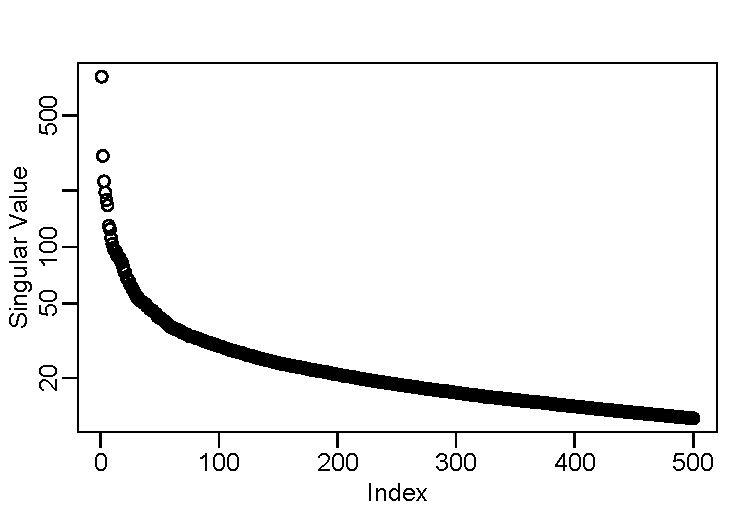
\includegraphics[width=4in]{figures/spectrum} }
 \vspace{0.2in}
 \end{figure}
   

 The conversion of words into principal components (singular vectors) produces
 a qualitative change in
 the significance of the regressors.  Figure \ref{fig:lsatstats} summarizes the
 $|t|$-statistics from a regression using the first 1,000 LSA  features
 in the same format as Figure \ref{fig:wordtstats}).  As with words, the model
 includes a polynomial in the length of the listings.   Sorting based on singular value is far more
 useful for ranking predictors than sorting on word frequency:  significant regressors  concentrate among the leading principal components, and these explain more variation than individual words. Unlike regression on
 frequencies of word types,  magnitudes of the 
 $t$-statistics decline roughly monotonically, with the most
 significant effects present in the initial components. Some signal remains in the smaller components; the slope in the
 half-normal plot for smaller coefficients is 1.9.  The fitted model with all 1,000 
 components obtains $R^2 = 0.756$
 with \prs = 0.664, compared to \prs = 0.580 for the previous regression on
 1,089 words.  Consequently, with more signal in the earlier components, $AIC_c$
 finds a more predictive model with fewer coefficients than needed for
 individual words.  The sequence of $AIC_c$ statistics for this model lies well
 below that for the regression on word frequencies in Figure \ref{fig:aic}.
  $AICc$ selects the model with 728 components, obtaining $R^2 = 0.734$
 and $\prs = 0.668$.
 
\begin{figure}
\caption{  \label{fig:lsatstats}  
  {\sl Absolute $t$-statistics from the regression of log prices on the first 1,000 LSA components from $\widetilde{W}$ with row and column weighting.}  }
  \centerline{ 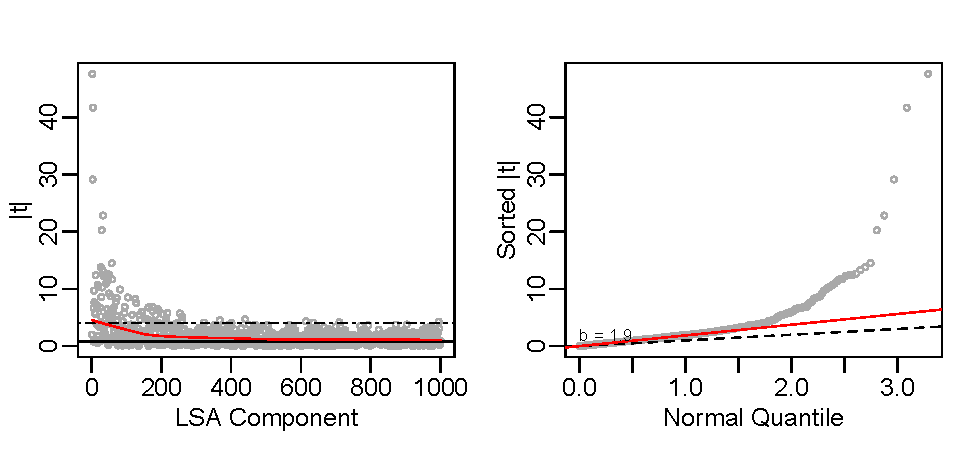
\includegraphics[width=5in]{figures/lsa_tstats.pdf} }
\end{figure}



 
%--------------------------------------------------------------------------
\section{Token Space}
\label{sec:tokenspace}
%--------------------------------------------------------------------------

 Token space is the vector space generated by modeling the sequence of word
 tokens as indicator vectors.  From this perspective, the frequencies in the
 document-word matrix $W$ are seen to be proportional to estimated covariances between random variables
 that represent different word tokens. Token space should feel
 familiar to statisticians and provides motivation and heuristics for
 creating a wide range of features from text.


\subsection{Words to Matrices} % ---------------------------------------------
\label{sec:cca}

 Recall that we observe $n$ real-estate listings that we will now generically
 call `documents'.  The \ith document is a sequence of $n_i$ word tokens 
 chosen from a vocabulary of $m$ word types.  To distinguish word types
 from word tokens, we use the symbol $\omega$ to denote types and $w$ to denote
 tokens.  We model each document as an independent observation of a stochastic
 process $H(\theta)$ that produces a sequence of word tokens.
  The \ith\ document is $\{w_1, w_2, \ldots, w_{n_i}\}$ with
 words chosen from the vocabulary, $w_i \in V$.  The stochastic process for each document 
 potentially has its own parameters $\theta_i$.  Section \ref{sec:topic} gives an example of such a
 process.  The word tokens within a document may be independent in some
 applications, but some dependence is common \citep[\eg][]{fosterkakade07}.
 We use $\ell$ to denote the concatenation of the observed tokens into a single list,
\begin{equation*}
   \ell = \left\{ \underbrace{w_{11},\,w_{12},\ldots,w_{1n_1}}_{\mbox{doc 1}},\,
            \underbrace{w_{21},\ldots,w_{2n_2}}_{\mbox{doc 2}}, \,
            \ldots, \underbrace{w_{n1},\ldots,w_{nn_n}}_{\mbox{doc }n} \right\}\;,
\end{equation*}
 with length $N = \sum n_i$.  The tokens resemble
  longitudinal data in which, for example, we observe a varying number
 of blood pressure measurements per subject in a medical trial.
 The subjects are usually modeled as independent,
 but the repeated measurements are not.  There is also another similarity. It is not uncommon in observational medical records to find that
 the number of measurements is correlated with health; sicker
 patients with more visits to the physician are more closely observed than those who are healthier.  In our data, longer sequences of tokens are associated with higher prices.


 Token space represents the list $\ell$ as a very sparse matrix
 defined by columns that indicate the chosen word types.  
 From $\ell$, define the $N \times m$ matrix
 $X$ in which $X_{ij} = 1$ if the \ith word token in $\ell$ is of type $\omega_j$:
 \begin{equation}
   X_{ij} = \left\{ \begin{array}{cc}
                   1 & \mbox{ if } \ell_i = \omega_j \cr
                   0 & \mbox{otherwise.}
                \end{array} \right.
 \end{equation}
 This conversion produces a large, sparse matrix with a single 1 in each row:
 \begin{equation}
  X =  \left( \rule{0em}{8em} \right.
  \begin{array}{cccccccc}
            \mbox{\scriptsize $\omega_1$} &
            \mbox{\scriptsize $\omega_2$} &
            \mbox{\scriptsize $\omega_3$} &
            \mbox{\scriptsize $\omega_4$} &
            \mbox{\scriptsize $\omega_5$} &
            \mbox{\scriptsize $\omega_6$} &   \cdots &
            \mbox{\scriptsize $\omega_m$}  \cr
            0  & 0 & 1 & 0 & 0 & 0 & \cdots & 0 \cr
            0  & 0  & 0 & 0 & 1 & 0 & \cdots & 0 \cr
             &&&  \vdots &&&&                                 \cr
            0  & 1  & 0 & 0 & 0 & 0 & \cdots & 0 \cr \hline
            0  & 0 & 0 & 0 & 1 & 0 & \cdots & 0 \cr
              &&&  \vdots &&&&                                 \cr
            1  & 0 & 0 & 0 & 0 & 0 & \cdots & 0 \cr \hline
              &&&  \vdots &&&\ddots&                                 \cr
              \\
           \end{array}
        \left. \rule{0em}{8em} \right)
          \begin{array}{c}
         \cr \mbox{\scriptsize{doc 1}} \cr \cr \cr \cr \mbox{\scriptsize{doc 2}} \cr \cr \vdots
  \end{array}
        \;.
    \label{eq:X}
 \end{equation}
 Clearly, this matrix is equivalent to the original text.


 This conversion produces more than numbers.  It also changes the way we
 interpret common summaries such as word frequencies. Though a trivial
 conversion, this representation of text converts the modeling of text into the analysis of
 sparse numerical matrices.  The document-type
 matrix $W$ used in LSA, for instance, is seen to be proportional to an estimated
 covariance matrix.  Let the $N \times n$ matrix $L$ identify the documents,
\begin{equation}
  L =  \left(  
           \begin{array}{ccccc}
            1  & 0 & 0 & \cdots & 0 \cr
            1  & 0 & 0 & \cdots & 0 \cr
             &&  \vdots &&                       \cr
            1 & 0 &  0 & \cdots & 0 \cr \hline
            0 & 1 & 0  & \cdots & 0 \cr
              &&  \vdots &&                        \cr
            0 & 1& 0 & \cdots & 0 \cr \hline
              &&  \vdots  &\ddots&             \cr
            0 & 0& 0 & \cdots & 1 \cr \hline        
           \end{array}
         \right) = I_n \otimes \one{n_i}  \;,
\end{equation}
where $\one{n}$ denotes a column vector of $n$ 1s. (This definition abuses the Kronecker product by allowing the right-hand vectors to have unequal length.)  Because we model the document length $n_i$ as the random outcome of the underlying process $H(\theta_i)$, $L$ also denotes an observed collection of random variables.  It is more compact to record these lengths as integers, but in token space, we model the random characteristics as vectors in $\R^{N}$.  The document-word matrix $W$ is then $N-1$ times the uncentered sample covariance matrix between the columns of $X$ and $L$, $W =  L'X$.


Once we think of $W$ as a covariance matrix, it becomes natural to associate LSA with canonical correlation analysis (CCA) rather than PCA.  In order for the SVD of $W$ to produce canonical vectors, however, we have to standardize the columns of $L$ and $X$.  Let 
\begin{equation}
  S_L = L'L/(N-1) = \mbox{diag}(n_i) \quad \mbox{ and  } \quad S_X = X'X/(N-1)
\label{eq:SL}
\end{equation}
denote the uncentered covariance matrices defined by $L$ and $X$, respectively.   As shown in the appendix, the SVD of $S_L^{-1/2} W S_X^{-1/2}$  yields the coefficients that define a CCA.  Standardizing $L$ is easy because $S_L$ is diagonal (when $L$ is uncentered), but $S_X$ is not.  To avoid computing and inverting $X'X$, we treat its columns as orthogonal and use the approximation $\widetilde{S}_X = \mbox{diag}(m_j)$, with $m_j$ counting the number of tokens of word type $\omega_j$. The resulting regressors are the left singular vectors of  $S_L^{-1/2} W \widetilde{S}_X^{-1/2} = \widetilde{W}$ defined in equation \eqn{Wtij}, matching the weighed principal components defined in Section \ref{sec:regrUsingLSA}.    This connection provides some further intuition behind the evident success of LSA in producing regressors.  The singular vectors of $\widetilde{W}$ are the coefficients that define the canonical variables of CCA.  The leading left singular vector identifies the linear combination of documents (columns of $L$) that is most correlated with a linear combination of words (columns of $X$).  If we imagine the elements of this singular vector being 0/1, then in this heuristic sense the CCA identifies clusters of documents associated with different collections of word types. 


\subsection{ Bigrams and Other Contexts } % ------------------------------------------
\label{sec:bigram}

A variety of other featurizations can be represented in token space. The sequential nature of the rows of $X$ suggests ideas from time series analysis, particularly lagged variables.  For instance, we might find interesting patterns in the association between adjacent word types.  Let $X_{-1}$ denote the lag of $X$ obtained by inserting a leading row of zeros and removing the final row.  Rather than use the document matrix $L$ to define the context of a word, this featurization uses the prior word.  The counts that produce the covariance between $X$ and $X_{-1}$ define the bigram matrix $B$,
 \begin{equation}
   B = X_{-1}' X   \;.
  \label{eq:B}
\end{equation}
(Note that the collection of word types we use includes a marker for the end of a document. Hence the counts in $B$ do not include pairs determined by the last word of one document and the first word of the next.) The use of a lagged indicator introduces a very different sense of context.  The SVD of $W$ identifies word types that appear together within the context of documents.  $B$ identifies word types used similarly within the narrow, very local context defined by the prior word. It is worth pointing out another difference.  $W$ ignores word placement (sequencing) within a document, treating a document as a bag of words.  In contrast $B$ combines the documents and relies on the sequence of word tokens. 

 
To make use of the bigram matrix, we proceed as in LSA and construct features from the leading singular vectors of $B$ obtained by random projection.  Let $\widetilde{U}_{B,k}$ denote the leading $k$ singular vectors obtained from the approximate SVD of the standardized bigram matrix $S_X^{-1/2} B S_X^{-1/2}$.   Each row of $\widetilde{U}_{B,k}$ represents a word type as a point in $\R^k$.   To build features for regression, we simply locate each document at the average position of its words, $\mbox{diag}(1/n_i)\,L'\widetilde{U}_{B,k}$.
The columns of  $\widetilde{U}_{B,k}$ are sometimes called ``eigenwords'' because of the way in which they form directions in word space \ras{cite lyle or someone using this name}.  Figure \ref{fig:bigramtstats} shows the $|t|$-statistics from regressing real estate prices on the document centroids computed from the leading 1,000 singular vectors of the bigram matrix.  The properties of these estimated coefficients resemble those of the coefficients obtained when using word counts as features (Figure \ref{fig:wordtstats}).  The estimates lack the concentration of signal into the leading components observed for LSA components (Figure \ref{fig:lsatstats}).  It should not be surprising, then, to find that bigram centroids perform similarly to words as predictors of price (Figure \ref{fig:aic}).  The minimum $AIC_c$ occurs when using 1,110 bigram centroids, for which \prs = 0.600.  This is higher than reached by simply using the word frequencies (0.580), but inferior to the fit produced by fewer LSA components (0.622).

 
\begin{figure}
\caption{  \label{fig:bigramtstats}  
  {\sl Absolute $t$-statistics from the regression of log prices on the first 1,000 bigram centroids.}  }
  \centerline{ 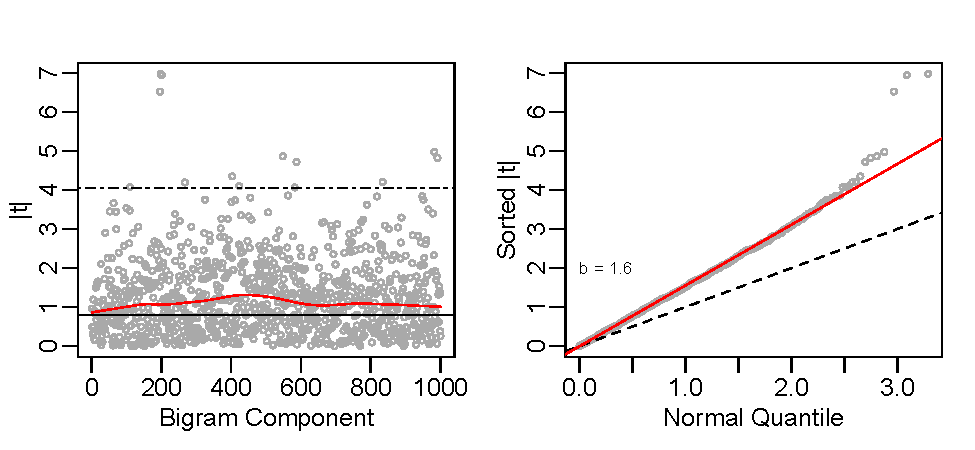
\includegraphics[width=5in]{figures/bigram_tstats.pdf} }
\end{figure}


The different contexts that produce either word frequencies or bigram counts offer some explanation for why LSA fares better in our analysis than features constructed from bigrams.  The context for words defined by the document matrix $L$ suggests that $W$ emphasizes semantic similarity, whereas the narrow context of adjacency provided by $X_{-1}$ suggests $B$ emphasizes syntax.   The document-specific context provided by $L$ is most natural -- and effective -- in our application.  For other tasks, such as predicting parts of speech, however, singular vectors constructed from bigrams are more effective.  As an example of this application, Figure \ref{fig:pos} shows word clusters defined by singular vectors of a bigram matrix  (eigenwords) constructed from  \ras{which is?}.  These eigenwords cluster word types by how they are used in language.  Nouns are distinct from verbs, adjectives, and \ras{what are the pos in the figure}.  


\begin{figure}
\caption{  \label{fig:pos}  
  {\sl Word clusters produced by singular vectors of the bigram matrix defined from \ras{insert} identify nouns(symbol), verbs(symbol)}, \ras{etc}. }
  %  \centerline{ 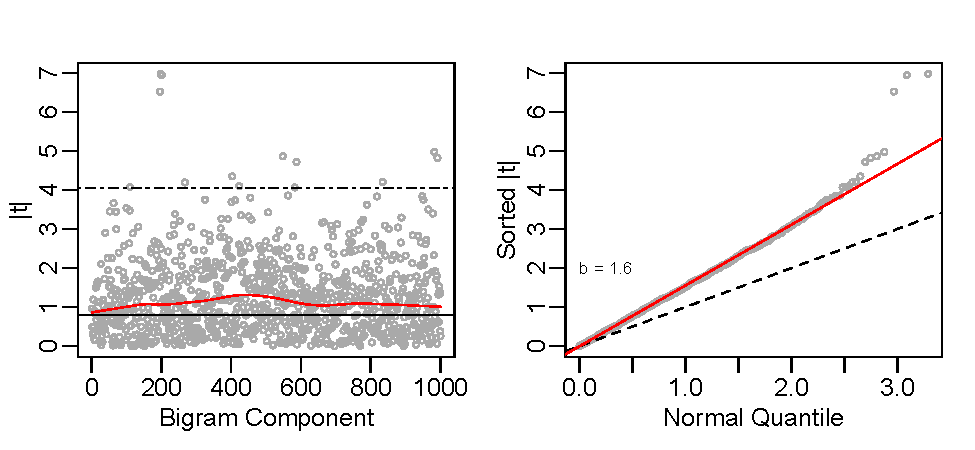
\includegraphics[width=5in]{figures/bigram_tstats.pdf} }
  \ras{Need version of the pretty plot using symbols rather than colors (at some point).}
\end{figure}


%--------------------------------------------------------------------------
\section{Topic Models}
\label{sec:topic}
%--------------------------------------------------------------------------


A class of generative probability models known as topic models offers an explanation for the success of the regressors we construct from text.  Topic models are common in the Bayesian analysis of text. \citet{blei12} provides a recent survey.   Topic models for text propose that the observed text of a document was produced by sampling words according to a mixture of distributions associated with the topics in the document.  Each topic is a probability distribution over a vocabulary of words.  Topic models treat words as exchangeable and model the text of a document as a multiset,  as in LSA.  In machine learning, topic modeling is  an unsupervised algorithm used to cluster documents based on the presence of latent topics revealed by a hierarchical Bayesian model. 


By incorporating a regression structure,  \citet{bleimcauliffe07} developed supervised topic models (called sLDA, for supervised latent Dirichlet allocation) in an application that is similar to ours.  Begin with the assumption that the observed text was produced by sampling words from $K$ topics. Let $P_j$ denote the vector of probabilities over words in the vocabulary that defines the \ith[j]\ topic.  Arrange these distributions as the $K$ rows of the $K \times m$ matrix $P$.  The sLDA model assumes that  the following algorithm generates the text of each document.  In particular, this algorithm fills in the elements of the response $Y$ and the token-space matrix $X$ defined in \eqn{X}:
\begin{enumerate}
 \item Let $\theta_i \sim \mbox{Dirichlet}(\al)$ be a $K$-vector that allocates the proportions of
          the $K$ topics that appear in the \ith\ document.  The parameter $\al$ is estimated in sLDA.
 \item Let $x_{ij}$ denote the row of $X$ associated with word $w_{ij}$.
    \begin{enumerate} 
      \item Independently sample one topic, $\tau_{ij} \sim \mbox{Multinomial}(1, \theta_i)$. 
               $\tau_{ij}$ is a $K$-vector with a single 1 that identifies the chosen topic for the \ith[j]\ word and
               is otherwise 0.
       \item Draw the vector $x_{ij} \sim \mbox{Multinomial}(1, \tau_{ij}'P)$.
    \end{enumerate}
  \item Sample the response $y_i \sim N(\tau_i'\beta, \sigma_\ep^2)$, where $\tau_i = \sum_j \tau_{ij}$.  The
           parameters $\beta$ and $\sigma_\ep^2$ are estimated within the sLDA modeling.
\end{enumerate}
Note that \citet{bleimcauliffe07} use the proportion of topics $\tau_i/n_i$ in the regression model rather the sum.  We use the sum here in order for this generative model to capture the evident association between document length and the response shown in Figure \ref{fig:parsed}.  Authors of listings write more about valuable properties than cheaper properties, and are motivated to write more about expensive properties, those with numerous attractive attributes worth mentioning.  

 
LSA is well-matched to this generative process because both treat a document as a bag-of-words with the expected response determined by a linear function of the underlying mixture of attributes.  Let $T$ denote the $n \times K$ matrix with rows $\tau_i$.  Then we can write the expected value of $W$ as a sum of $K$ outer products:
\begin{equation}
    \ev W = T\, P = \sum_k T_k \, P_k' \;,
  \label{eq:EW}
\end{equation}
where $T_k$ is the \ith[k]\ column of $T$, enumerating the presence of the \ith[k]\ topic in the various documents.  This factorization of $\ev W$ mimics the structure of the SVD of $W$.  For our models of text, the left singular vectors $U_W$ from \eqn{Wk} capture the allocation of attributes over documents, recovering much of the information in $T$.  Of course, there are many ways to factor a matrix, and it is not apparent why the factorization provided by the SVD would produce good estimates of this factorization.  For instance, the right singular vectors of $W$ do not necessarily define a stochastic matrix.  Obtaining good regressors, however, does not require that we recover $P$ or $T$.  We need only recover the range of $T$ in order to predict the response.  


\subsection{Examples of Simulated Data} %-------------------------------------------------

The following two examples illustrate the performance of LSA methods when applied to data generated by the sLDA process.  Each example uses $n = 5,000$ documents with words chosen from a vocabulary of $m = 1,500$ words. The lengths of the documents are exogenous to the sLDA algorithm; we set  the lengths in our simulations to $n_i \sim \mbox{Poisson}(50)$.  The simulation generates the response and text of these documents by sampling $K = 30$ topics, with $\theta_i = 0.4$ throughout. This parameter produces documents that mix several topics.  For the response, we sampled the regression coefficients $\beta \sim N(\mu=2,\sigma^2=1)$; allowing a few negative coefficients produces a slightly weaker correlation between the response and document length. In our simulations, the correlation is about 0.25.  To finish the generation of the response, we chose the errors variance $\sigma_\ep^2$ in step 3 so that  $R^2 =0.60$ in the  regression of $y$ on the true topic composition in $T$.  


The two examples are distinguished by the degree of overlap among the 30 topic distributions.  In both cases, we simulated distributions by sampling a Dirichlet distribution, $P_k \sim \mbox{Dirichlet}(\alpha)$. Small values of $\alpha$ produce very 'spiky' distributions with little overlap; increasing $\alpha$ produces distributions with substantial common support.   Figure \ref{fig:P} graphs probability distributions with $\alpha = 0.01$ (essentially disjoint) and $\alpha = 0.10$.  All but one of the points in the left frame with $\alpha=0.01$ lie along the axes of the graph; the two distributions are essentially singular.  In contrast, with $\alpha=0.10$, both distributions assign  probability to many words in common.


\begin{figure}
\caption{ \label{fig:P}
{ \sl  Probability distributions over words simulated from a Dirichlet distribution with parameter $\al = 0.01$ (left) are essentially disjoint, whereas with $\al = 0.10$ (right), the simulated distributions substantial common support.}}
 \centerline{
 \vspace{0.1in}
 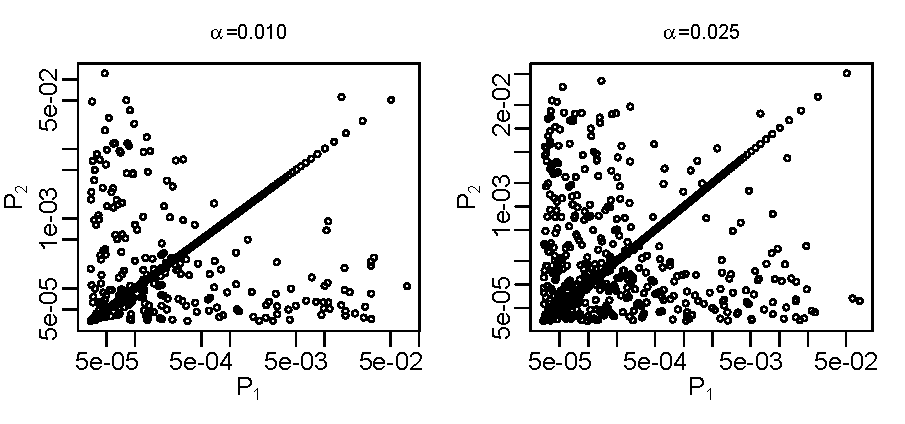
\includegraphics[width=7.5in]{figures/P} }
 \end{figure}


 One of our reasons for simulating data from  a probability model  was to gain some insight as to the best normalization to apply to $W$ prior to performing LSA.  First, we simulated documents with nearly disjoint topic distributions ($\al = 0.01)$.  Figure \ref{fig:spectra} shows the first 100 singular values produced by two normalizations of $W$, either none (raw frequencies) or the approximate CCA normalization $S_L^{-1/2}WS_X^{-1/2}$. The results do not produce a clear-cut winner. The gap between adjacent singular values at $K=30$ is most pronounced with the CCA normalization, though evident in both situations. This more noticeable gap favors the CCA normalization, but this normalization simultaneously flattens the spectrum.  In both cases, the leading singular value stands out. Without normalization, the first left singular vector $U_1$ picks up document length, and the first right singular vector $V_1$ captures word frequency.  The CCA normalization weakens these patterns.  In the case of data produced by overlapping topics ($\al = 0.10$), neither spectrum produces the slightest hint of a gap.
 
\begin{figure}
\caption{ \label{fig:spectra} 
{ \sl Spectra obtained for the document/word matrix $W$ with no standardization or CCA standardization.}}
 \centerline{
 \vspace{0.1in}
 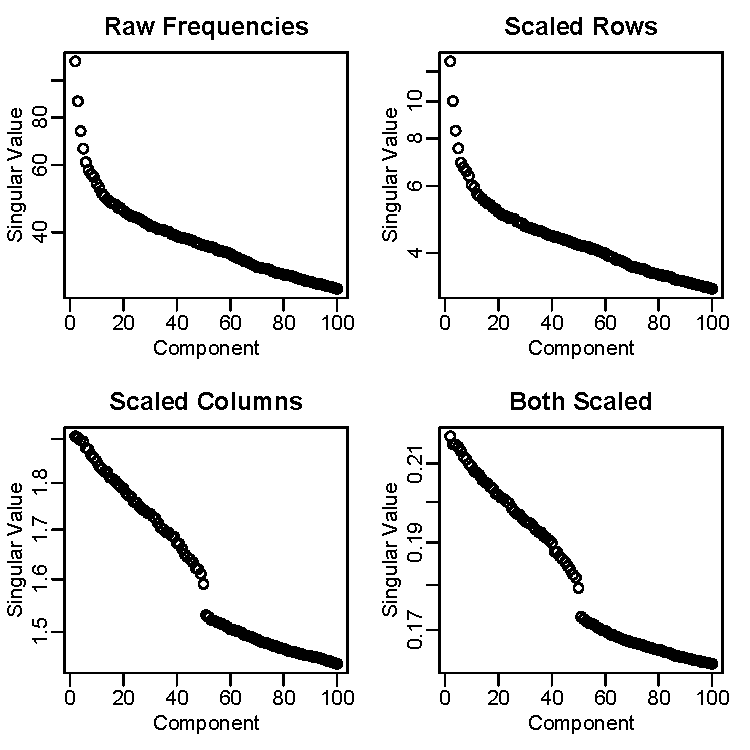
\includegraphics[width=6.0in]{figures/spectra} }
 \end{figure}


Our objective in modeling text, however, is not to determine the precise number of latent variables (as if these exist in actual text), but rather lies in building regression models.  For this task, CCA  standardization produces a better set of regressors.  Table \ref{fig:ccawins} summarizes the predictive $R^2$ of regression models fit to 100 samples produced by the sLDA algorithm.  As in the prior examples, the population has $K=30$ topics that are either distinct ($\al=0.01$) or overlapping ($\al=0.10$).  The error variance in the regression of $Y$ on $T$ is chosen to produce a model with $R^2 = 0.60$.  In each case, we fit $k=100$ singular vectors or, in the case of word frequencies, the frequencies of the most common 200 words.  When the topics are distinct,  CCA regressors produces an average \prs\ equal to XXXX, which is nearly as good as the best possible, namely that produced by the smaller number of unobserved topics themselves.  The unnormalized singular vectors do well, but lag behind with an average \prs\ at XXXX.  Using raw frequencies is lower still.  When the topics are overlapping, the results for all of these data-driven features fall off.  The average \prs\ for the CCA singular vectors drops down to XXXX, compared to XXXX for the unnormalized singular vectors.  The performance of word counts falls even more to XXXX.

\begin{table}
\caption{ \label{tab:ccawins} 
{ \sl Average predictive $R^2$ statistics for regression models fit to simulated data generated by the sLDA model.}  Results summarize a simulation of 100 replications with distinct ($\al = 0.01$) and overlapping ($\al = 0.10$) topic distributions. Standard errors are XXXX }
 \begin{center}
  \begin{tabular}{lcc}
                                                      &  \multicolumn{2}{c}{Dirichlet Parameter} \cr
   \multicolumn{1}{c}{Regressors}&  $\al = 0.01$   & $\al = 0.10$  \cr \hline
   Latent topics $T$                       &   0.600 & 0.606  \cr
   CCA standardized  ($k=100$)   &  0.561  & 0.437  \cr
   Not standardized ($k=100$)      & 0.470  & 0.368  \cr
   Most frequent 200 word counts  & 0.395 &  0.124   \cr \hline
   \end{tabular} \end{center}
 \end{table}


%--------------------------------------------------------------------------
\section{Variable Selection and Cross Validation}
\label{sec:cv}
%--------------------------------------------------------------------------


For comparison, we performed repeated 10-fold transductive cross validation.  Transductive cross-validation presumes that the full collection of regressors is available for the training data, which in this case implies that we have all of the data available to perform the principal components analysis.  Only the values of the response are hidden in each fold of the cross-validation; the collection of regressors is fixed.  We repeated the 10-fold cross-validation 20 times, each time randomly partitioning the cases into 10 folds. The observed average squared error was slightly higher than anticipated at $0.614 \pm 0.007$, but basically agreed with the estimate from the fitted model. 


%--------------------------------------------------------------------------
\section{Lighthouse Variables and Interpretation}
\label{sec:light}
%--------------------------------------------------------------------------
 
 

 Our emphasis on predictive accuracy does not necessarily produce an
 interpretable model, and one can use other data to create such structure.  Our
 explanatory variable resemble those from principal components analysis and
 share their anonymity.  To provide more interpretable regressors, the presence
 of partial quantitative information in real estate listings (\eg, some listings
 include the number of square feet) provides what we call ‘lighthouse variables’
 that can be used to derive more interpretable variables.  In our sample, few
 listings (about 6\%) indicate the number of square feet.  With so much missing
 data, this manually derived predictor is not very useful as an explanatory
 variable in a regression.  This partially observed variable can then be used to
 define a weighted sum of the anonymous text-derived features, producing a
 regressor that is both complete (no missing cases) and interpretable.  One
 could similarly use features from a lexicon to provide more interpretable
 features.


Though regression models are seldom causal, one is often tempted to interpret
 properties of the solution within the domain of application.  Because the
 predictors computed from the decompositions in the prior section describe
 subspaces rather than some specific property of words, interpretation is
 essentially non-existent.


 To obtain features that are interpretable, we exploit the pre<sence of
 characteristics that are occasionally observable.  For example,
 most home listings do not include the number of bathrooms.  An
 explanatory variable obtained by parsing this count is missing for 74\% of the property listings.  We can use this partially observed variable, however, to construct a more interpretable variable from either the principal components of $W$ or the bigram variables.  


 Let $z \in \Rn$ denote the partially observed or perhaps noisy data
 that measures a substantively interesting characteristic of the
 observations.  For our example, $z$ is the partially observed count of the number of bathrooms.  Rather than use $z$ directly as a predictor of $y$, we
 can use it to form an interpretable blend of, for instance, $U_W$.   In
 particular, we simply regress $z$ on these columns, finding the
 linear combination of these basis vectors most correlated with the
 observed variable.  This variable, call it $\hat{z}$ then becomes
 another regressor.  Because such variables can be used to guide the
 construction of interpretable combinations of the bases $U_W$ and
 $C$, we call these lighthouse variables.  
 
 
 In our example, the correlation between the number of bathrooms and the price of the listing is 0.42 for listings that show this characteristic.  This correlation is much smaller (0.19) if we fill the missing values with the mean number of bathrooms (Figure  \ref{fig:parsed}).  If we form the projection $\hat{z}$ given by regressing the observed counts on the corresponding rows of $U_W$, this new regressor has correlation 0.29 with the log of price.



%--------------------------------------------------------------------------
\section{Summary and Next Steps}
\label{sec:disc}
%--------------------------------------------------------------------------
  
  Regression modeling always benefits from greater substantive insight, and the modeling of text is no exception.  An obvious approach to building regressors from text data relies on a
 substantive analysis of the text.  For example, sentiment analysis constructs a
 domain-specific lexicon of positive and negative words.  In the context of real
 estate, one might suspect  words such as ``modern'' and ``spacious''  to be associated with more expensive properties, whereas
 ``Fannie Mae'' and ``fixer-upper'' to signal properties with lower prices.  The
 development of such lexicons has been an active area of research in sentiment
 analysis over the past decade \citep{taboada11}.  The development of a lexicon
 require substantial knowledge of the context and the results are known to be
 domain specific.  Each new problem requires a new lexicon.  The lexicon for
 pricing homes would be quite different from the lexicon for diagnosing patient
 health.  Our approach is also domain specific, but requires little user input
 and so can be highly automated.


 Our analysis here shows that one can exploit well-known methods of multivariate analysis to create regressors from unstructured text.  Compared to iterative methods based on MCMC, the computations are essentially immediate.  Surprisingly, the resulting regressors are quite predictive in several examples we have explored.  For example, we used this same methodology to model ratings assigned to wines based on tasting notes.  The tasting notes themselves are typically shorter than these real estate listings (averaging about 42 tokens compared to 72 for the listings), but we have a larger collection of about 21,000.  Using the methods demonstrated here, a regression using 250 principal components of $W$ explains about 66\% of the variation in ratings, we a remarkably similar distribution of effect sizes as shown in Figure \ref{fig:wine}.  Similarly, regression on the 250 left and 250 right regressors constructed from the bigram matrix explains about 68\% of the variation.  We plan to explore other applications in the near future.
 
 
 \begin{figure}
 \caption{ \label{fig:wine} \sl Regression t-statistics from a model that predicts wine ratings using 250 principal components of $W$ based on 21,000 wine tasting notes.}
 
 \centerline{
   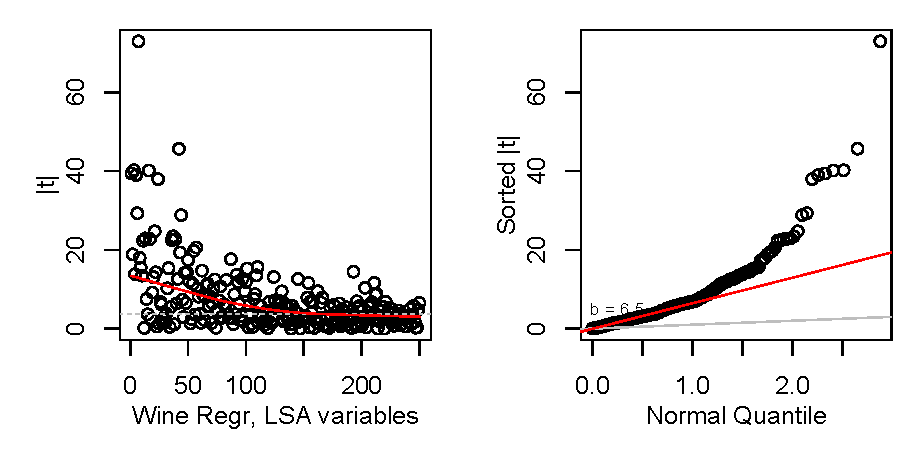
\includegraphics[width=4in]{figures/wine.pdf}
   }
  \end{figure} 
  
  
   The connection to topic models is an important aspect of these results.  Topic models define a DGP for which the regressors that we construct capture the underlying data-generating mechanism.  If one accepts topic models as a reasonable working model of the semantics of text, then it is no accident that regressors constructed from text are predictive.


 Our work here merely introduces these methods, and we hope that this introduction will encourage more statisticians to engage problems in  modeling text.  Our results here also suggest several directions for further research:

   \begin{description}
   
   \item[n-grams.]  Our example uses bigrams to capture word associations captured by adjacent placement.  Other reasonable choices define different measures of context,  such as trigrams (sequence of 3 words) or skipped bigrams (words separated by some count of tokens).  Some preliminary results show, for instance, that trigrams offer modest gains, albeit at a nontrivial increase in computation.
   
   \item[Transfer learning.]  Transfer learning refers to learning what can be extrapolated from one situation to another.  In our context, it would be of interest to learn how well models developed from data in June 2013 work when applied to data from later time periods or different locations.  It is evident that the models shown here would not perform so well applied to the language of a different market, such as in Miami or Los Angeles.  Not only do the characteristics of valuable properties change, but  local conventions for phrasing listings are also likely to be different.  Having a methodology for distinguishing idiosyncratic local features from those that generalize in time or space would be valuable. 
   
  \item[Alternative forms of tokenization.] Would be interesting to explore the use of stemming to reduce the number of word types and with a larger collection of documents, to explore annotation (that would distinguish words by their part of speech).  Further parsing, lexical analysis.  Some readers will be troubled by the simplicity of the  bag-of-words representation of a document.  Our methods understand neither the English language nor the rules of grammar and spelling.  They do not attempt to untangle  multiple uses of the same word.  Linguists have debated the ability of such  representations to reveal the meaning of language, and it is clear that the bag of words representation loses information.  Just imagine cooking from``bag of words'' recipe or following a ``bag of words'' driving directions.  Nonetheless, this very direct representation produces very useful explanatory variables within our application.  We leave open the opportunity to embellish this approach with more domain specific methods of parsing, such as adding part-of-speech tags and lexical information.
   
   \item[Use of unsupervised data.] Most words are used only once or twice, meaning that we lack enough data to identify their connection to the response or indeed to other words.  As a partial remedy, it may be possible to build regressors that represent such words from larger, more generic text such as the collection of n-grams collected by Google.  Using this supplemental unsupervised data requires solving the problem of transfer learning, at least to some degree, but opens the door to much more extensive examples. 
   
   \item[Variable selection.]  The distribution of effects (such as shown by the $|t|$ statistics of the text-derived regressors) are poorly matched to the so-called `nearly black' model commonly adopted in research on the theory of variable selection.  Rather than have most of the predictive power concentrated in a very small number of regressors, these regressors spread the power of many.  
      
   It would also be interesting to explore these models for nonlinearity. Variable selection is perhaps unnecessary for using the regressors derived from $U_W$ and $C$, but essential if one hopes to detect and incorporate nonlinearity. In particular, searching for nonlinearity -- such as interactions -- requires variable selection.  Even a very large corpus of documents looks small compared to the number of possible second-order interactions.  Finally, the ordered presentation of the $|t|$ statistics suggests an opportunity for variable selection derived from alpha investing \citep{fosterstine08}.  Alpha investing is a procedure for testing a sequence of hypotheses that benefits from {\it a priori} ordering of the tests.
   
      \item[Sparse CCA.] If the left singular vectors were sparse, only 0/1, then the heuristic explanation could become less heuristic and more honest.  Would sparse CCA (Witten et al) be useful? \citet{witten09}


   \end{description}

One can generalize LSA from words and documents to collections of other items,
 such as phonemes in speech or tones in music \cite[called latent semantic
 mapping in][]{bellegarda05}.



%--------------------------------------------------------------------------
\section*{Acknowledgement}
%--------------------------------------------------------------------------

The authors thank Vanessa Villatoro from Trulia's PR Team for allowing us to scrape the data from their web site.

%--------------------------------------------------------------------------
\section*{Appendix}
%--------------------------------------------------------------------------

 The singular value decomposition can produce either a
 PCA or CCA.  The role of the SVD for computing principal components is both
 well documented and direct.  The left singular vectors are the principal
 components, and the right singular vectors provide the loadings (or coefficients).  The use of
 the SVD for CCA is implicit and known \citep[e.g.][]{fosterkakade07} but more
 subtle, and so we provide the details here.

 Let $X$ and $Y$ denote column-centered matrices of observed random
 variables of dimension $n \times k_x$ and $n \times k_y$, respectively, with
 $k_x \le k_y$. The sample variance-covariance matrices are
 \begin{displaymath}
   S_{xx} = X'X/(n-1),\quad S_{yy} = Y'Y/(n-1), \quad \mbox{ and }
   S_{xy} = X'Y/(n-1) = S_{yx}' \;.
 \end{displaymath}
 For simplicity, assume both $X$ and $Y$ are full rank so that $S_{xx}$ and
 $S_{yy}$ are invertible.  The first pair of canonical variables are the linear
 combinations, say $X a_1$ and $Y b_1$, which are most highly correlated,
 \begin{displaymath}
   a_1, b_1 = \arg \max_{a \in \R^{k_x},b \in \R^{k_y}} \corr(Xa,Yb) \;.
 \end{displaymath}
 The second pair, $X a_2$ and $Y b_2$, defines the linear combinations that are
 most correlated with each other, but orthogonal to $Xa_1$ and $Yb_1$.  Let $A$
 denote the $k_x \times k_x$ with columns $a_1,\ldots,a_{k_x}$ and let $B$ be
 the corresponding matrix with columns $b_1,\ldots,b_{k_y}$.  The coefficients of
 the canonical variables are obtained by solving the eigenvalue problems
 \begin{eqnarray}
   S_{xx}^{-1} S_{xy} S_{yy}^{-1} S_{yx} \, A &=& A \, \Lambda_A \cr
   S_{yy}^{-1} S_{yx} S_{xx}^{-1} S_{xy} \, B &=& B \, \Lambda_B      
 \label{eq:appA}
 \end{eqnarray}
 The leading $k_x$ elements of the diagonal matrices $\Lambda_A$ and $\Lambda_B$
 are the squared canonical correlations between $X$ and $Y$.  The canonical
 variables are the leading $k_x$ columns of $X\,A$ and $Y\,B$.


 The SVD provides an alternative method of computation. Define the standardized,
 orthogonal variables
 \begin{displaymath}
   \tilde{X} = X S_{xx}^{-1/2} \quad \mbox{and }  \quad
   \tilde{Y} = Y S_{yy}^{-1/2} 
 \end{displaymath}
 with covariance matrix
 \begin{displaymath}
   \tilde{S} =
     \cov(\tilde{X},\tilde{Y}) = S_{xx}^{-1/2} S_{xy} S_{yy}^{-1/2} \;.   
 \end{displaymath}
 Let the matrix $U$ hold the left singular vectors of $\tilde{S}$.  These are
 eigenvectors of $\tilde{S} \tilde{S}'$, satisfying
 \begin{equation}
    S_{xx}^{-1/2} S_{xy} S_{yy}^{-1} S_{yx} S_{xx}^{-1/2} \, U = U \, \Lambda_U \;.
 \label{eq:appS}
 \end{equation}
 If we multiply both sides of \eqn{appS} by $S_{xx}^{-1/2}$ then we see that
 $S_{xx}^{-1/2}U$ solves the first equation of \eqn{appA} with $S_{xx}^{-1/2}U = A$.
  Similarly, if $V$ denotes the right singular vectors of $\tilde{S}$, then
 $S_{yy}^{-1/2}V = B$.  Notice that the left and right singular vectors of
 $\tilde{S}$ are the coefficients that define the canonical vectors.  Unlike PCA,
 in which the SVD gives the principal components, for CCA the SVD gives the
 canonical coefficients, not canonical variables.

%--------------------------------------------------------------------------
% References
%--------------------------------------------------------------------------

\bibliography{../../../references/stat,../../../references/TextPapers/text}
\bibliographystyle{../bst/ims}

\end{document} %==========================================================
